\chapter{Alternativas arquitecturas}
\label{anexo-a}
% TODO: Explicar como expliqué a Javier en el correo las alternativas de las arquitecturas y los pros y contras de cada una de ellas y el por qué de la decisión

En el proceso de diseño de la arquitectura software del proyecto se evaluan distintas opciones con el objetivo de seleccionar la más adecuada para cumplir con los objetivos y requisitos de la empresa. Los principales motivos de este análisis son:

\begin{itemize}
    \item Tener o no un middleware que actúe de servidor web para comunicar la aplicación web y la aplicación existente de Ibernex (Helpnex).
    \item El problema de compatibilidad de utilizar SignalR (Véase  \hyperref[anexo-b]{Anexo B}) para comunicar la aplicación de Ibernex y la aplicación web.
\end{itemize}

En un principio, el diseño de arquitetura propuesto por la empresa es el que se puede ver en la \textit{Figura A.1}. 

\begin{figure}[!h]
    \centering
    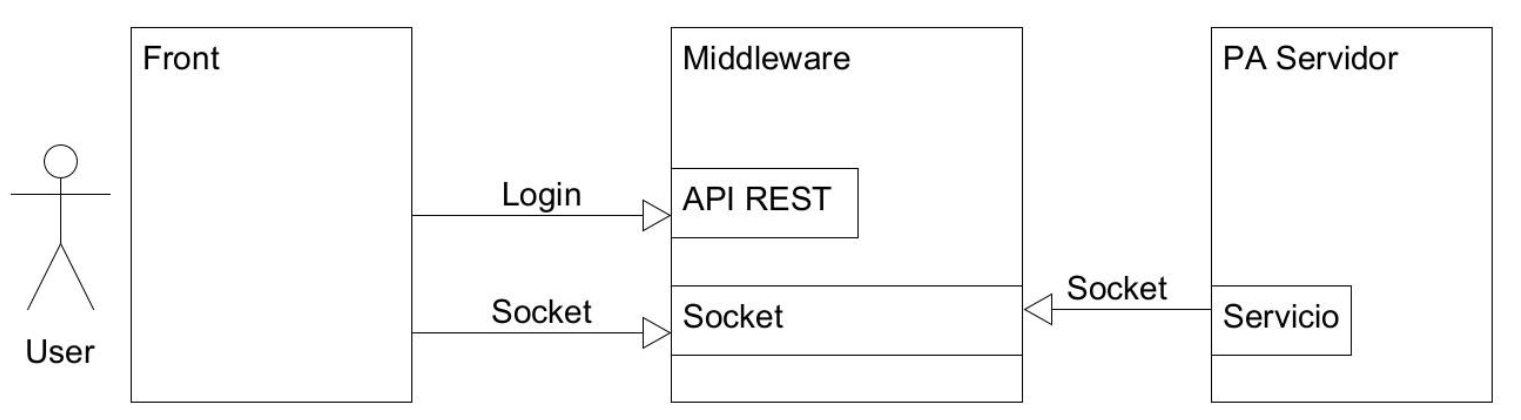
\includegraphics[width=15cm]{Imagenes/Descripcion-arquitectura}
    \caption{Diagrama propuesto por la empresa}
    \label{fig:descripcion-arquitectura}
\end{figure}

\begin{figure}[!h]
    \centering
    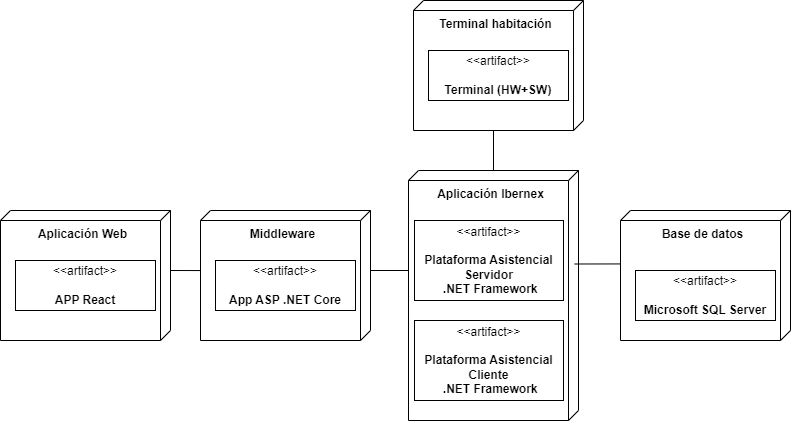
\includegraphics[width=15cm]{Imagenes/Arquitectura-despliegue-2}
    \caption{Diagrama de despliegue con Middleware}
    \label{fig:despliegue-2}
\end{figure}


\begin{figure}[!h]
    \centering
    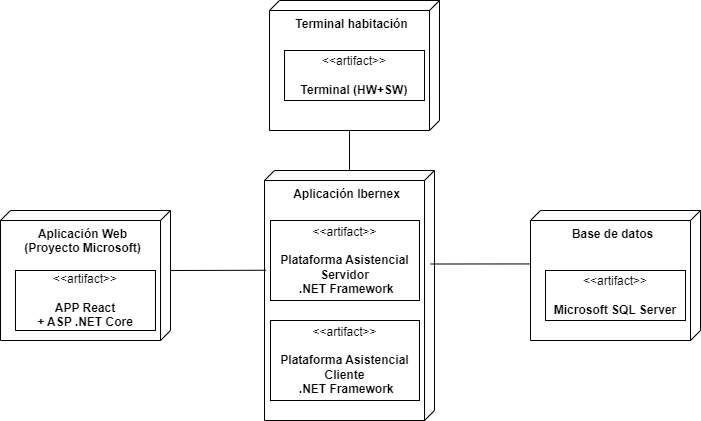
\includegraphics[width=15cm]{Imagenes/Arquitectura-despliegue-3}
    \caption{Diagrama de despliegue - único proyecto}
    \label{fig:despliegue-3}
\end{figure}


La arquitectura elegida para el proyecto es la que se puede ver en la \hyperref[fig:despliegue]{\textit{Figura 2.1}} que se encuentra en una de las secciones anteriores.



